% Technical report - QSMPC-QKD-QHE-AI-Hybrid
% Build: xelatex -interaction=nonstopmode technical-report.tex  (twice, for the ToC)
% Tables, macros and figures under generated/ are produced by build_data.py and build_figures.py
% from live artefacts, so no number in this document is transcribed by hand.
\documentclass[11pt,a4paper]{article}

% pdflatex + lmodern rather than fontspec: Latin Modern is not installed as a system font here,
% and xelatex silently fell back to nullfont, producing a PDF whose pages rendered but whose text
% did not. A build that "succeeds" with no glyphs is exactly the kind of green-but-wrong signal this
% report is about, so the toolchain is pinned to what is actually present.
\usepackage[T1]{fontenc}
\usepackage{lmodern}
\usepackage[margin=2.4cm]{geometry}
\usepackage{booktabs}
\usepackage{longtable}
\usepackage{graphicx}
\usepackage{xcolor}
\usepackage{amsmath}
\usepackage{caption}
\usepackage{enumitem}
\usepackage{fancyhdr}
\usepackage[hidelinks]{hyperref}

\definecolor{accent}{HTML}{2B6CB0}
\definecolor{warn}{HTML}{C05621}
\captionsetup{font=small,labelfont={bf,color=accent}}
\setlist{itemsep=1pt,topsep=3pt}

\pagestyle{fancy}\fancyhf{}
\lhead{\small QSMPC-QKD-QHE-AI-Hybrid}
\rhead{\small Technical Report \gitsha}
\cfoot{\small\thepage}
\renewcommand{\headrulewidth}{0.3pt}

\newcommand{\gitsha}{7f82ae3-dirty}
\newcommand{\reportdate}{29 October 2026}
\newcommand{\npublished}{11}
\newcommand{\nchecklistrows}{631}
\newcommand{\nchecklistlines}{4{,}706}
\newcommand{\nusecases}{5}
\newcommand{\ndefectclasses}{21}


\title{\vspace{-1.4cm}\textbf{A Quantum-Safe Orchestration Layer with\\Client-Side Encrypted Inference}\\[3pt]
\large Architecture, measured results, and a verification methodology\\that produced \ndefectclasses{} defect classes}
\author{Technical Report, revision \texttt{\gitsha}}
% Generated into macros.tex from the HEAD commit date. It was a literal and went stale by
% three days; a report whose every table is generated should not hand-maintain its own date.
\date{\reportdate}

\begin{document}
\maketitle
\thispagestyle{fancy}

\begin{abstract}
\noindent
This report describes a research proof-of-concept that chains post-quantum key establishment,
quantum key distribution simulation, secure multiparty computation and CKKS homomorphic encryption
into a single orchestration layer, and evaluates privacy-preserving machine learning across
\nusecases{} industry use cases. The public demonstrator performs its homomorphic linear algebra and
its garbled-circuit non-linearities \emph{in the browser}, so its cryptographic timings are measured
client-side rather than asserted. \npublished{} models are published with pinned revisions.

The contribution we consider most transferable is not the architecture but the verification
methodology. Over several rounds it produced \ndefectclasses{} distinct classes of silent defect --- a
constant-class predictor whose accuracy exactly equalled the majority-class rate, an inverted
diagnostic label map that made the demonstrator display the opposite of the model's output, a
shuffled-\texttt{DataLoader} label misalignment statistically indistinguishable from random,
and a baseline cited from the correct paper but the wrong table, among others. Each was invisible to
tests, type checks and aggregate metrics. Section~\ref{sec:wrong} tabulates all \ndefectclasses{} and
states four in full, alongside four conclusions the authors published and subsequently retracted.

We report what the system measures, what it does not, and where its numbers are not comparable to
the published baselines they sit beside.
\end{abstract}

\vspace{-2mm}
\noindent\rule{\textwidth}{0.4pt}
\begin{small}
\textbf{Scope and status.} Research proof-of-concept, not a production system. Real implementations
where tractable, explicitly labelled simulation where not. Licence Apache-2.0. This document reports
measurements produced by the code at revision \texttt{\gitsha}; every table is generated from the
repository's own artefacts at build time rather than transcribed.
\end{small}
\noindent\rule{\textwidth}{0.4pt}

\tableofcontents
\newpage

\section{Summary}
This report documents a research proof-of-concept and, more usefully, the verification methodology
applied to it. The system chains post-quantum key establishment, a quantum-key-distribution
simulation, secure multiparty computation and CKKS homomorphic encryption, and runs privacy-preserving
inference for \nusecases{} industry use cases entirely in the visitor's browser. \npublished{} models
are published at pinned revisions.

Headline results: the encrypted tier reproduces its plaintext teacher exactly on one use case
(AUC-PR 0.9681 for both) and falls well short on another (AUC 0.7882 against 0.9147), so no single
``encryption costs $X$'' figure would be honest. \ndefectclasses{} classes of silent defect were
found in a system with green tests, and four previously published conclusions were retracted after
further measurement. Structure follows ANSI/NISO Z39.18-2005 (R2010) --- Summary, Introduction; Methods,
Assumptions and Procedures; Results and Discussion; Conclusions --- with one deliberate departure:
the defects and retractions are given their own section rather than being folded into Limitations.
No standard blesses a ``negative results'' heading, and Limitations is the conventional home for
them; they are separated here because they are a principal result of this work rather than a
qualification on one.

\section{Introduction and scope}

\subsection{Problem}
Post-quantum migration is a procurement deadline before it is a research problem. NIST FIPS 203, 204
and 205 have been final since August 2024; NIST IR 8547, still an initial public draft, would deprecate
112-bit-strength public-key algorithms such as RSA-2048 after 2030 and disallow all quantum-vulnerable
ones, P-256 included, after 2035; and for national security systems only, CNSSP 15 requires CNSA 2.0
algorithms in new acquisitions from 1 January 2027. Harvest-now-decrypt-later makes the confidentiality
deadline earlier than the signature deadline for any data with a long secrecy lifetime.

Separately, privacy-preserving computation has become tractable for \emph{small} models. Homomorphic
evaluation remains cost-bounded --- a recent systematisation puts private LLM inference at roughly
four orders of magnitude slower than plaintext, and reports that only about 20\% of surveyed systems
are model-preserving. So a project that wants both a genuine industry model and genuine encryption
has two honest options: shrink the model until it fits the cipher, or state plainly that the
cryptographic demonstration runs on something smaller than the headline model.

\subsection{What this system is}
This project takes the second option and makes the cost measurable. Each use case carries two model
tiers: a T2 \emph{teacher} --- the real architecture, plaintext --- and a T1 \emph{student}, small
enough to evaluate under CKKS, distilled from the teacher's own output. The gap between them is
reported as a first-class metric rather than elided.

\subsection{What is new here, and what is not}
This project's own verification rule is that a novelty claim must survive an adversarial search for
prior art. Applied to its headline claim the answer is asymmetric, and reporting only the flattering
half would be the kind of omission the rest of this document exists to avoid.

\textbf{MPC in a browser is not new.} webSPDZ (IACR ePrint 2025/487) compiles MP-SPDZ to WebAssembly
and communicates over WebRTC or WebSockets, and it names JIFF and MPyC-Web as earlier browser MPC
engines. The garbled-circuit half of this system re-implements a known idea.

\textbf{Homomorphic \emph{evaluation} in a browser is where the search returned nothing.} Every
artefact located encrypts client-side and evaluates server-side. IACR ePrint 2026/515 defines
``client-side operations'' as encryption and decryption while \emph{users offload large computations to
servers}; Zama's TFHE-rs WebAssembly API documents support for key generation, encryption and
decryption but \emph{not} FHE computation, citing WASM threading and a 2\,GB memory ceiling. This
system evaluates a real CKKS dot product and a real CKKS convolution in the tab.

\textbf{The claim is therefore the composition rather than either half}: PQC key establishment, then
a simulated QKD link (it yields a key length, not key bytes), then secure multiparty computation, then
homomorphic evaluation, then model inference --- chained end to end in one browser tab with no server-side compute. A search for an
integrated browser system performing that whole chain returned nothing. Two caveats travel with the
claim and are stated wherever it appears: the two MPC parties are notional, running over an in-memory
transport within a single tab, so the protocol, the bytes and the wall-clock are real while the party
separation is not; and the quantum channel is simulated, because no browser API for quantum
communication exists. Client-side execution is also not automatically private --- WWW 2026's WAMO
paper argues that browser deployment moves a model into a hostile environment, which is among the
reasons the models here are published openly rather than treated as secrets.

\subsection{What this system is not}
It does not claim quantum \emph{advantage}. The measured quantum-kernel and variational classifiers
lose to a RandomForest baseline on the same data, and the registry records
\texttt{quantum\_beats\_classical: false} rather than omitting the comparison. The value proposition
is quantum-\emph{safety}, which is regulation-driven and dated.

\section{System architecture}

\subsection{Layers}
Four workstreams share one pipeline and a crypto-agility registry:
\begin{itemize}
  \item \textbf{WS1 --- AI-QKD.} BB84 two-intensity decoy-state simulation with GLLP tagged-fraction
        accounting, a selectable E91/CHSH protocol, a quantum-measurement QRNG with SP~800-90B
        continuous health tests and a Leftover-Hash-Lemma extractor.
  \item \textbf{WS2 --- QML intrusion detection.} Eight classes (seven QKD attack types plus normal
        traffic), scored on macro F1 rather than attack-versus-normal F1.
  \item \textbf{WS3 --- QSMPC.} Shamir secret sharing with $d$-level QFT secure summation, quantum
        oblivious transfer, quantum-safe private set intersection.
  \item \textbf{WS4 --- QHE and AI.} CKKS linear layers with MPC non-linearities, including a genuine
        homomorphic convolution (im2col into \texttt{dot\_plain}).
\end{itemize}

\subsection{Crypto-agility as an architectural property}
Every algorithm is resolved from a registry and selected before a run. There is no in-band
negotiation and no silent fallback: this is crypto-agility in the EU NIS Cooperation Group sense ---
modular design enabling component replacement --- and deliberately not cipher-suite negotiation
during protocol execution.

\begin{table}[htbp]\centering\small
\caption{Cryptographic parameters as configured}
\begin{tabular}{lll}
\toprule
\textbf{Layer} & \textbf{Primitive} & \textbf{Note} \\
\midrule
KEM & \texttt{ML-KEM-768 + X25519} & FIPS 203 hybrid; ct 1088 B \\
Signature & \texttt{ML-DSA-65} & FIPS 204; sig 3309 B \\
FHE & \texttt{CKKS, ring degree 8192} & 4096 slots, one multiplicative level per dot product \\
MPC & \texttt{Garbled circuits (emp-wasm)} & non-linear layers: ReLU, argmax \\
QKD & \texttt{BB84 two-intensity decoy} & GLLP tagged fraction \\
\bottomrule
\end{tabular}
\end{table}


\subsection{The slot budget, which is the real constraint}
A CKKS ring of degree 8192 provides 4096 slots, and a ciphertext-plaintext dot product costs one
multiplicative level. Parameter count is therefore \emph{not} the binding budget; slot width is.
Section~\ref{sec:featuremap} shows what that distinction bought once it was recognised.

\section{Machine learning methodology}

\subsection{Teacher-student distillation, and what is reported}
Students are fitted against the teacher's own output rather than ground truth, so
\texttt{agreement} measures substitution rather than two independent fits that happen to correlate.
Fidelity and task performance are reported separately because they decouple empirically: in one case
agreement rose from 0.8841 to 0.9471 in Round 24 while the task metric did not move at all. The current value is 0.9829; the pair is quoted as a before/after, not as today's figure. Reporting one as
though it were the other is a category error this project made and corrected.

\subsection{Metric selection}
Four of the five verticals have a documented failure mode in which the obvious aggregate looks
healthy while the class that matters is not learned. Each headline metric is therefore the one the
relevant literature reports, with the flattering companion printed beside it:

\begin{itemize}
  \item \textbf{Finance:} minority-class F1 at a 1-in-981 positive rate. The precision-recall
        baseline is $P/(P{+}N)\approx0.001$, so an ROC-AUC of 0.95 says nothing.
  \item \textbf{Satellite:} event-wise $F_{0.5}$ under an overlap rule. Point-adjusted F1 is computed
        \emph{only} to show its inflation --- under point adjustment ``even a random anomaly score can
        easily turn into a state-of-the-art TAD method'' (Kim \emph{et al.}, AAAI 2022).
  \item \textbf{Medical:} AUC, with the majority-class rate and the number of distinct classes
        predicted printed alongside (Section~\ref{sec:wrong} explains why).
\end{itemize}

\subsection{Operating-point selection by net benefit}
\label{sec:netbenefit}
The screening operating point is chosen by net benefit,
\[
  \mathrm{NB}(p) \;=\; \frac{\mathrm{TP}}{N} \;-\; \frac{\mathrm{FP}}{N}\cdot\frac{p}{1-p},
\]
in which the subtracted term is the exchange rate the threshold itself declares. Three criteria were
tried and two rejected on measurement:

\begin{itemize}
  \item \textbf{F1 --- rejected, degenerate.} When discrimination is weak, minority-class F1 is
        maximised by calling everything positive: recall goes to 1 while precision falls only to the
        base rate. The criterion selected the extreme grid point and the resulting model predicted
        the positive class for all 156 test images. The validation score it chose, 0.4242, is exactly
        the all-positive value $2p/(1+p)$ at $p=0.269$. This is a theorem, not a local surprise ---
        Lipton et al.\ (2014) prove that an uninformative classifier's F1-optimal behaviour is to
        classify every example as positive.
  \item \textbf{Youden's $J$ --- rejected, symmetric.} $J$ cannot be gamed the same way, but it is
        the symmetric special case: it prices a missed cancer and a false alarm equally, which no
        screening programme does and which this project had never stated.
  \item \textbf{Net benefit --- adopted.} It makes the exchange rate explicit and places the model on
        the same axis as treat-all and treat-none, so ``worse than not screening'' is visible rather
        than inferred.
\end{itemize}

\begin{figure}[h]\centering
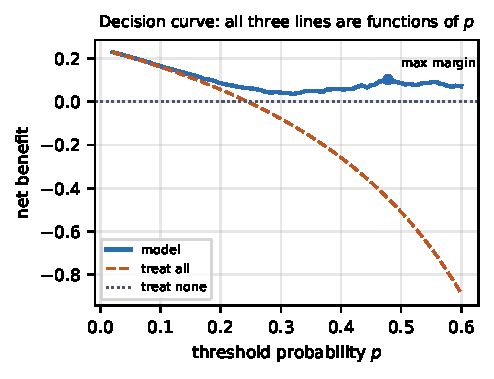
\includegraphics[width=0.48\textwidth]{generated/fig_decision_curve.pdf}
\hfill
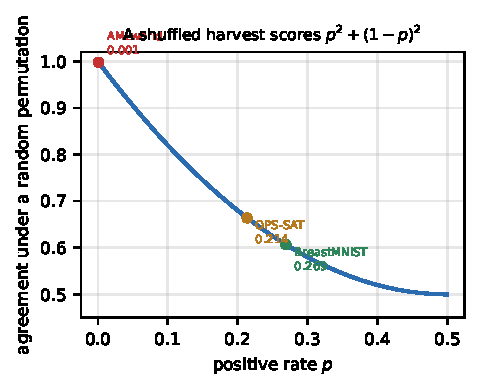
\includegraphics[width=0.48\textwidth]{generated/fig_permutation_null.pdf}
\caption{\textbf{Left:} a decision curve. All three lines are functions of $p$, and only matched-$p$
comparisons are meaningful --- an error the authors made and corrected
(Section~\ref{sec:wrong}, W8). \textbf{Right:} agreement expected from a randomly permuted label
harvest, $p^2+(1-p)^2$. At a 1-in-981 positive rate a completely broken pairing scores 0.998, which
is why an alignment check with a ``near 1.0'' pass condition cannot detect misalignment on an
imbalanced task.}
\end{figure}

\subsection{Client-side feature expansion under encryption}
\label{sec:featuremap}
A polynomial expansion of the input is a function of the \emph{plaintext}, so the client computes it
before encrypting and the encrypted step remains a single packed dot product at unchanged
multiplicative depth. For the OPS-SAT segment classifier this expands 19 features to 209 --- well
inside the 4096-slot budget --- and measurably improved the encrypted tier:

\begin{center}\small
\begin{tabular}{lccc}
\toprule
& linear & quadratic & paired bootstrap 95\% CI on the delta \\
\midrule
minority-class F1 & 0.8649 & \textbf{0.9043} & $[+0.0154,\ +0.0929]$ \\
AUC-PR            & 0.9275 & \textbf{0.9681} & $[+0.0089,\ +0.0853]$ \\
\bottomrule
\end{tabular}
\end{center}

Both intervals exclude zero over 4000 paired resamples, so the gain survives at this sample size.
The interval is wide --- its lower bound is a fifth of the point estimate --- so the defensible claim
is ``a real improvement of at least about one AUC-PR point'', not the point estimate.

Three qualifications belong with that result. The technique is \emph{not novel}: the mathematics is
a known explicit feature map, and placing feature construction at the client-side plaintext boundary
specifically to bound homomorphic depth is published system design. Depth is unchanged but cost is
not zero --- slot-summation rotations rise from $\lceil\log_2 19\rceil = 5$ to
$\lceil\log_2 209\rceil = 8$ key-switches. And the client must know the feature map, which discloses
model \emph{structure} though not weights.

Applied to the finance student the same change \emph{lowered} the headline metric, so it is a
per-model flag rather than a default. That negative result is recorded in the flag's own help text.

\section{The five use cases}

Each use case exercises the full chain --- post-quantum key establishment, key distribution,
a privacy-preserving computation, and an inference --- but they were chosen so that the
\emph{computation} differs, not merely the data. A demonstrator in which five verticals run the same
pipeline over five CSV files would show nothing about the cryptography.

\subsection{Finance: anti-money-laundering with cross-institution set intersection}
Two institutions need to know whether a counterparty appears on both watchlists without disclosing
either list, so the privacy primitive is quantum-safe private set intersection, and the inference is
a fraud score computed under CKKS. The corpus is IBM AMLworld HI-Small: 5{,}078{,}345 transactions
at one laundering event in 981, evaluated on a strictly temporal split with the decision threshold
tuned on a third window the model was never fitted on.

The gap to the published baseline is the largest in the project and its cause is architectural
rather than a tuning failure. The reference implementation computes per-transaction subgraph
patterns over a dynamically updated graph; this project computes per-account scalar aggregates. A
degree is one number per account; the reference feature is a pattern match in that transaction's own
neighbourhood at the moment it arrives. An earlier note attributed the gap to a proprietary licence
and to truncated multi-hop reachability. The licence is real but was never the mechanism, and the
reachability claim did not survive arithmetic: the source paper decomposes its own contribution and
caps multi-hop cycle features at about 4\% relative, against more than 30\% for fan-in/fan-out,
which this project already implements.

Investigating that gap found a genuine defect. Per-account aggregates were computed over the whole
training window, so a training row's feature included activity that happened after it while test
rows received the same table as a stale snapshot. Making the aggregates causal --- each row sees only
strictly earlier edges --- raised minority-class F1 from 0.0808 to 0.1519. Leakage was disproved
rather than argued: every feature is bit-identical whether or not later rows exist.

\subsection{Healthcare: federated training with encrypted diagnosis}
Hospitals train jointly without pooling records, so the primitive is secure aggregation over
federated updates, and the inference is a genuine homomorphic convolution --- im2col into a CKKS
\texttt{dot\_plain}, with ReLU and argmax evaluated under MPC. This is the only use case where the
encrypted path evaluates a convolutional model rather than a linear one.

It is also where the most serious defects were found, and all of them were in the \emph{measurement}
rather than the cryptography: a constant-class predictor, an inverted diagnostic label map, and a
label/sampler misalignment. Section~\ref{sec:wrong} treats them in full. The current encrypted
student reaches AUC 0.7882 against its teacher's 0.9147, with accuracy above the majority-class rate
and both classes predicted.

\subsection{Genomics: pooled allele counts by secure summation}
Research sites contribute allele counts without revealing per-site genotypes, using $d$-level QFT
secure summation. This use case deliberately reports \emph{no} AUROC: the reference panel carries no
case/control status, so the quantity is undefined, and printing a plausible number for it would be
the single most tempting error available here. What is computable from real genotypes is the
ancestry portability gap, and that is reported instead, because it is the clinically important
finding rather than a substitute for the missing one.

\subsection{Telecom and defence: intrusion detection on quantum-channel telemetry}
Eight classes --- seven attack types plus normal traffic --- scored on macro F1, because
attack-versus-normal F1 would let a detector that recognises one common attack look competent. Both
a classical RandomForest and quantum classifiers are trained on identical data, and the classical
baseline wins: macro F1 0.9866 against 0.8316 for the quantum-kernel SVC and 0.4667 for the
variational classifier. The registry records \texttt{quantum\_beats\_classical: false}. Reporting
this is the point of running both.

\subsection{Satellite: free-space QKD with direct telemetry}
A downlink under real loss, with an inline eavesdropper check, and anomaly detection over multi-year
ESA telemetry. The secrecy criterion is the one place where a familiar constant proved actively
misleading. A threshold of 0.11 reproduces the textbook loss-free case, and the deeper derivation
gives a capacity
\[
  C_s \;=\; Q_{\text{Bob}}\bigl[\,1 - h(e) - g\,h(e_x + e_z)\bigr],
  \qquad g = 10^{\,\text{loss\_dB}/10},
\]
in which the loss term dominates; $g$ counts the channel and the detector, not the station's optics.
On the 800\,km downlink (32.2\,dB of channel loss, 27.3\,dB from Eve to Bob's detector, $g \approx 533$)
the admissible error rate falls from 0.11 to about $6.5\times10^{-5}$ --- three orders of magnitude, and
in the permissive direction, so the constant would have declared links secure that are not. The scalar
was replaced by the computed capacity.

The downlink itself is Micius's, read value by value from Liao et al.\ (2017), with the atmosphere
scaled by air mass from 5.5\,dB at 1200\,km and no link below 10 degrees of elevation. Integrated over
Liao's pass of 19 December 2016 and counted as the paper counts --- signal states only --- it gives the
measured detections and sifted bits within 1\,percent. A second tab models what carries a key past the
horizon: the trusted satellite relay Micius flew between Xinglong and Graz, and a plane of satellites
linked to their neighbours.

The key is the composable finite key of one pass peaking at the page's range, the block every flown
experiment found computes its key on: Lim et al.'s (2014) bound for a source that sends the vacuum,
on the pass's counts summed second by second. On Liao's pass at their failure probability of
$10^{-9}$ it gives 164,183 bits, 0.55 of the 300,939 they report; on the Micius--Zvenigorod session
it gives 0.56 of a key computed with Chernoff bounds, the same gap on a second pass, so it is the
analysis and not the channel. The same bound reproduces Rusca et al.'s (2018) two-decoy figures to
within a factor of 2.5, always below them, and their ratio to the one-decoy figures within
15\,percent. Pooling passes, or a time held at one range, are offered beside it; at 800\,km a key
needs about 33\,s of link time, which one range of a low orbit does not hold.

\section{Security model and its boundaries}

\subsection{What is real and what is simulated}
The distinction is load-bearing and is stated per component rather than in aggregate:

\begin{center}\small
\begin{tabular}{lll}
\toprule
\textbf{Component} & \textbf{Status} & \textbf{Basis} \\
\midrule
ML-KEM-768 + X25519 & real & library implementation, conformance-tested \\
ML-DSA-65 signatures & real & round-trip and tamper vectors \\
CKKS linear layers & real & node-seal, measured in the browser \\
Garbled-circuit argmax & real & Polytune 2PC, measured in the browser \\
BB84 decoy-state & \emph{simulated} & channel model, not hardware \\
QSDC secrecy capacity & \emph{computed} & closed form, loss-dependent \\
\bottomrule
\end{tabular}
\end{center}

Nothing labelled simulated is reported with a wall-clock timing that implies otherwise. The public
demonstrator performs no server-side computation at all, which is why its homomorphic and MPC
timings are meaningful: they are measured in the visitor's own tab.

\subsection{Conformance rather than happy-path testing}
Post-quantum library correctness is checked with negative vectors, not only round-trips. This
distinction was not academic. An earlier harness reported ten of ten passes on a negative-vector
suite whose negatives were wrong-\emph{length} inputs --- a test that any implementation passes by
rejecting malformed input, and which says nothing about arithmetic. Modulus vectors were decisive
where the original suite was not. Separately, a library upgrade reversed an argument order in its
signing API; type checking, the build and the full test suite all passed, and only the browser
surfaced it.

\subsection{Dependency currency, and a gap no scanner reports}
The homomorphic layer uses \texttt{node-seal}, a WebAssembly build of Microsoft SEAL. The pinned
dependency resolves to \texttt{node-seal} 7.0.0, whose vendored source declares \textbf{SEAL 4.1.2,
released 11 July 2024}. Upstream shipped \textbf{4.4.0 on 25 July 2026} described by its maintainers
as a critical security update hardening untrusted deserialization, then 4.4.1 and 4.4.3 in the first
week of August 2026. \emph{No CVE or advisory exists for either package}, so dependency scanners
report nothing and the lockfile is current against its own registry. The gap is findable only by
reading upstream release notes.

Whether it matters here depends on the architecture, and the answer is specific rather than
reassuring-by-default. The hardened surface is deserialization of untrusted input. This system
generates keys, encrypts, evaluates and decrypts entirely in the visitor's own tab, performs no
server-side computation, and deserialises no externally supplied ciphertext --- so that surface is
not reachable in this deployment. It would become reachable the moment any server component accepted
a ciphertext from a client, and that is recorded as a condition rather than a footnote.

The same reasoning governs a second upstream statement. SEAL's security documentation was revised in
July 2026 to state that its CKKS implementation targets IND-CPA and \textbf{not} IND-CPA-D, and that
noise flooding must be applied by the application before a decrypted CKKS value crosses a trust
boundary. Here the secret key, the decryption and the plaintext result are all in the same tab, so no
such boundary is crossed. The architecture is what makes this safe; the cipher alone does not.

\subsection{Known limitations of the threat model}
The client-side feature map used in Section~\ref{sec:featuremap} discloses model \emph{structure}
--- the identity of the expansion --- though not weights. Published work treats exactly this as a
problem worth solving with randomised shuffling. Where model confidentiality is part of a claim, the
disclosure must be stated; here it is, and the claim is not made.

\section{Results}
\label{sec:results}

\begin{table}[htbp]\centering\small
\caption{Published models: measured value against the baseline each is compared to. Tier T1 runs under encryption; T2 is the plaintext teacher. A dash means the model is declared in the registry but not trained in this build, which is reported rather than hidden. Dataset licences are given in full in the next table; this column names the corpus so the licence is never abbreviated.}
\begin{tabular}{llllll}
\toprule
\textbf{Model} & \textbf{Tier} & \textbf{Metric} & \textbf{Measured} & \textbf{Baseline} & \textbf{Dataset} \\
\midrule
\texttt{finance\_aml.student} & T1 & minority-class F1 (laundering) & 0.0614 & 0.6323 & IBM AMLworld HI-Small \\
\texttt{finance\_aml.gnn} & T2 & minority-class F1 (laundering) & -- & 0.6323 & IBM AMLworld HI-Small \\
\texttt{finance\_aml.gbm} & T2 & minority-class F1 (laundering) & 0.1519 & 0.6323 & IBM AMLworld HI-Small \\
\texttt{genomics.prs} & T2 & AUROC (European ancestry) & -- & 0.6330 & PGS Catalog scoring files \\
\texttt{medical\_fl.student} & T1 & AUC & 0.7882 & 0.9010 & MedMNIST v2 BreastMNIST \\
\texttt{medical\_fl.resnet18} & T2 & AUC & 0.9147 & 0.9010 & MedMNIST v2 BreastMNIST \\
\texttt{medical\_fl.resnet50} & T2 & AUC & 0.7988 & 0.8570 & MedMNIST v2 BreastMNIST \\
\texttt{satellite\_comms.student} & T1 & event-wise F0.5 & 0.0032 & 0.9680 & ESA Anomaly Dataset (ESA-ADB), Mission1 lightweight channels 41-46 \\
\texttt{satellite\_comms.opssat\_student} & T1 & AUC PR & 0.9681 & 0.9790 & OPS-SAT-AD \\
\texttt{satellite\_comms.telemanom} & T2 & event-wise F0.5 & 0.4545 & 0.9680 & ESA Anomaly Dataset (ESA-ADB), Mission1 lightweight channels 41-46 \\
\texttt{satellite\_comms.opssat} & T2 & AUC PR & 0.9681 & 0.9790 & OPS-SAT-AD \\
\texttt{telecom\_ids.student} & T1 & macro F1 (synthetic QKD-attack telemetry) & 0.9883 & -- & QKD attack telemetry (synthetic, methodology-grounded) \\
\texttt{telecom\_ids.transformer} & T2 & macro F1 across attack classes & -- & -- & CIC-IDS2017, Engelen-corrected redistribution (WTMC 2021) \\
\texttt{telecom\_ids.qml} & T2 & macro F1 (synthetic QKD-attack telemetry) & -- & -- & QKD attack telemetry (synthetic, methodology-grounded) \\
\texttt{telecom\_ids.nidd} & T2 & macro F1 across 9 network-attack classes & 0.9264 & -- & 5G-NIDD (Combined.csv) \\
\bottomrule
\end{tabular}
\end{table}


% Licences in their own table, printed whole. They were a column inside the models table above,
% rendered through split(";")[0][:22]; that removed the qualifier from three of the seven licences
% this report publishes, and a qualifier is what makes a licence string long, so the truncation was
% biased toward overclaiming. The models table now names the corpus and this one carries the terms.
\begin{table}[htbp]\centering\small
\caption{Dataset licences, quoted whole. An earlier revision printed this column inside the models table through split(";")[0][:22], which removed the qualifier from three of the seven licences that reach this report - and a qualifier is what makes a licence string long, so truncation is biased toward overclaiming.}
\begin{tabular}{>{\raggedright\arraybackslash}p{4.2cm}>{\raggedright\arraybackslash}p{9.5cm}}
\toprule
\textbf{Dataset} & \textbf{Licence, in full} \\
\midrule
5G-NIDD (BTS1\_\allowbreak{}BTS2\_\allowbreak{}fields\_\allowbreak{}preserved.csv) & CC-BY-4.0 \\
CIC-IDS2017, Engelen-corrected redistribution (WTMC 2021) & provider's own pages state conflicting terms \\
ESA Anomaly Dataset (ESA-ADB), Mission1 lightweight channels 41-46 & CC-BY-3.0-IGO \\
IBM AMLworld HI-Small & CDLA-Sharing-1.0 \\
MedMNIST v2 BreastMNIST & CC-BY-4.0 asserted by MedMNIST; the BUSI authors publish no licence \\
OPS-SAT-AD & CC-BY-4.0 \\
PGS Catalog scoring files & per-score; EMBL-EBI Terms of Use by default \\
QKD attack telemetry (synthetic, methodology-grounded) & no licence granted; synthetic rows generated by this repository's own code \\
\bottomrule
\end{tabular}
\end{table}


\begin{figure}[h]\centering
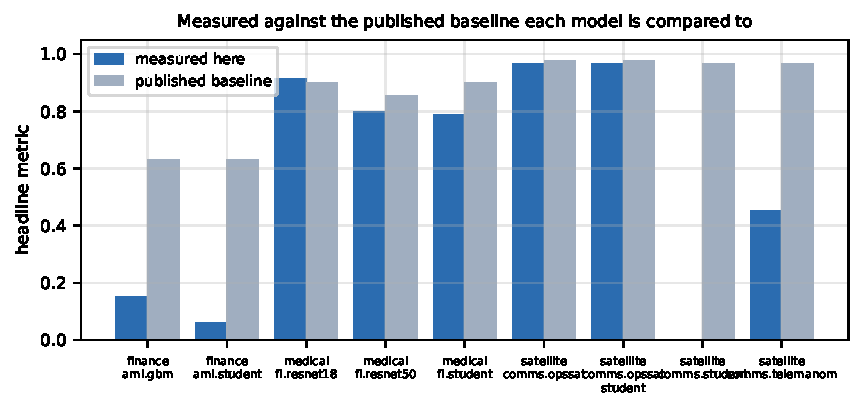
\includegraphics[width=0.95\textwidth]{generated/fig_baselines.pdf}
\caption{Measured value against published baseline. Two comparisons are deliberately not
like-for-like and are discussed below rather than presented as parity.}
\end{figure}

\subsection{Where the numbers are not comparable, stated explicitly}
\begin{itemize}
  \item \textbf{Satellite event-wise $F_{0.5}$ is computed over three labelled events.} The corpus
        contains 320 annotated intervals over the full timeline, but the annotated anomalies are
        concentrated early and a temporal split leaves three inside the scored window. Both recorded
        values decompose uniquely on three events, and the difference between two identical-configuration
        runs is exactly one extra false-alarm run. The reference partition holds 65 events. The
        number is reported with its denominator attached.
  \item \textbf{The reference metric is corrected; ours was not.} The benchmark multiplies event
        precision by the time-level true-negative rate, which is why most of its baselines read
        below 0.001. Both values are now computed.
  \item \textbf{Genomics reports no AUROC.} The reference panel has no case/control status, so the
        quantity is undefined and is not printed. What \emph{is} computable from real genotypes is
        the ancestry portability gap, which is the clinically important finding.
\end{itemize}

\subsection{The encrypted tier's cost}
The distilled students are 20 to 3{,}226 parameters. For the medical use case the encrypted student
reaches AUC 0.7882 against its teacher's 0.9147; for OPS-SAT the encrypted student matches its
teacher's AUC-PR exactly at 0.9681. The gap is therefore strongly task-dependent, and reporting a
single ``encryption costs $X$ percentage points'' figure across use cases would be misleading.

\section{What we got wrong, and how it was found}
\label{sec:wrong}

This section exists because the defects below were invisible to every automated signal the project
had. Shapes matched, losses decreased, tests passed, type checks passed, and aggregate metrics looked
plausible. Each was found by a specific act of measurement, and the check that would have caught it
is now a numbered row in the verification checklist (\nchecklistrows{} rows at this revision).

{\scriptsize
\begin{longtable}{p{2.5cm}p{5.2cm}p{6.2cm}}
\caption{Eight classes of silent defect, all found in a working system with green tests}\\
\toprule
\textbf{Class} & \textbf{What it was} & \textbf{Why nothing caught it} \\
\midrule
\endfirsthead
\toprule
\textbf{Class} & \textbf{What it was} & \textbf{Why nothing caught it} \\
\midrule
\endhead
\textbf{Constant predictor} & medical CKKS student emitted one class for all 156 test images & accuracy 0.7308 equalled the majority rate exactly; AUC 0.354, below random \\
\textbf{Inverted class labels} & four sites asserted the opposite of MedMNIST's own metadata & the demo displayed the opposite diagnosis to the model's output \\
\textbf{Sampler misalignment} & shuffled DataLoader output paired positionally with dataset order & teacher/ground-truth agreement 0.6227, inside the permutation null \\
\textbf{Wrong baseline row} & cited ESA-ADB Table 2 (all events) for an anomalies-only task & like-for-like row is Supplementary Table 9 at 0.968, not 0.786 \\
\textbf{Uncorrected metric} & reported uncorrected event-wise F0.5 against a corrected baseline & ESA-ADB multiplies event precision by the time-level TNR \\
\textbf{Licence divergence} & published artefact recorded ImageNet weights; two docs said random & publish now refuses any model whose manifest records a pretrained source \\
\textbf{Guard too narrow} & both\_scored\_zero required BOTH models at zero & teacher 0 vs student 0.0032 rendered as the encrypted model beating its teacher \\
\textbf{Manufactured margin} & treat-all evaluated at a different threshold from the model & a zero margin reported as +0.2308; caught by the degeneracy guard \\
\bottomrule
\end{longtable}}


\subsection{Four findings worth stating in full}

\paragraph{W1 --- A model that had learned nothing, with a respectable number.}
The medical CKKS student emitted a single class for all 156 test images. Its accuracy of 0.730769 is
exactly $114/156$, the majority-class rate, and its AUC was 0.354 --- below random. It was invisible
because the registry declared AUC as the model's headline while the record stored accuracy: AUC
would have been unmissable, accuracy read as ``behind but plausible''. The metric-name mismatch had
been on the backlog as a cosmetic registry inconsistency. It was the thing hiding the failure.

\paragraph{W3 --- Labels attached to the wrong images.}
Teacher labels were harvested through a \texttt{DataLoader} constructed with \texttt{shuffle=True} ---
correct for training, and the loader was also the training loader --- then paired positionally with
the dataset in its original order. Every distilled label landed on a different image. Measured
teacher/ground-truth agreement was 0.6227 where a sequential pass gives 1.0000; 4000 simulated
permutations give a 99\% interval of $[0.5641, 0.6484]$, so the harvest was statistically
indistinguishable from random. \texttt{predict\_loader} now refuses a random sampler outright.

Two rounds had attributed this student's weakness to CKKS capacity --- ``3{,}226 parameters is a
feasibility budget, not a diagnostic one'' --- and that explanation had been written into three
documents. Training the identical architecture on aligned labels scored 0.23 AUC higher, which
disproved it. The resulting rule: before concluding that the encrypted tier is small and therefore
weak, train the same small model properly once and see what it can do.

\paragraph{W8 --- A comparison that manufactured its own margin.}
The first implementation of net benefit scored the model across a threshold grid but evaluated
treat-all \emph{once} at the grid midpoint, reporting ``best $+0.2308$ at $q=0.050$ (treat-all
$-0.0150$)''. At $q=0.050$ the model flagged every validation case, so it \emph{was} treat-all, and
treat-all at that same threshold also scores $+0.2308$. The true margin was zero and the comparison
produced a win by moving the goalposts to a different $p$. It was caught because an unrelated guard
--- added earlier to reject any threshold collapsing to a single class --- refused to fold the
result.

\paragraph{W9 --- A label leak inside a published artefact, behind a pin that looked valid.}
The evaluation sample published alongside the finance model contained a single feature that
reproduced its label: every row with \texttt{hour\_of\_day} $\ge 3$ was laundering, at 100\%
precision. Anyone who downloaded the sample to reproduce the reported figure would have scored a
trivial threshold rule and read it as the model working. Three things had to fail together. The
sample was regenerated after the pin was recorded, and nothing invalidated the pin, so
\texttt{hf\_revision} still resolved and still looked current. The guard written to catch exactly
this was wrong twice --- first testing disjointness of unique values, which is meaningless on
continuous floats, then computing a binary rank AUC over multi-class labels and printing 5.1292, a
number outside $[0,1]$ that was not questioned. And the neighbouring use case escaped the guard
altogether because its \texttt{feature\_names} field held class names, so the guard iterated over
nothing and reported success.

The repository's own headline figure was never affected: it is computed over 1{,}523{,}504 rows that
the leaked sample never touched. An earlier draft of this section said the leak accounted for 13.8\%
of the model's headline number; that was wrong, and the 13.8\% belonged to the verification figure.
The correction matters more than the original claim, because a defect report that overstates its
blast radius is the same category of error as the defect. What the episode establishes is narrower
and worse: a guard that reports success without examining anything is indistinguishable, in a log,
from a guard that passed.

\subsection{Retracted conclusions}
Four published conclusions were withdrawn after further measurement:
\begin{enumerate}[label=(\alph*)]
  \item \textbf{``Seed variance.''} Two teacher AUCs were reported as moving on reruns ``with no
        functional change'', supported by a six-seed spread. The initialisation had changed, not the
        seed: the trainer defaulted to pretrained weights and the reruns omitted the flag. With it,
        both reproduce the documented figures to four decimal places.
  \item \textbf{``The student's ceiling is 0.0262.''} A threshold sweep was reported as proving
        capacity was the binding constraint, and a probe predicting three times that performance was
        recorded as having over-promised. The probe was right; the trainer was passing the teacher a
        scaler round-trip that is a mathematical no-op and not a numerical one. Fixing it moved the
        shipped student to 0.0614, above the asserted ceiling.
  \item \textbf{``The GPU is unusable for this work.''} Reported after
        \texttt{torch.cuda} raised ``no kernel image available'' on the training host, with the
        conclusion that the card's compute capability was unsupported. The measurement had been taken
        with the system interpreter, which carries a CUDA 12.1 build; the project's own virtual
        environment carries a CUDA 13.0 build that drives the same card correctly. The retraction
        keeps one real finding: the system interpreter reports
        \texttt{is\_available() == True} and then raises at the first kernel launch, so
        availability is not a capability check.
  \item \textbf{A regulatory date ``correction'' that was itself wrong.} A recorded compliance date
        was rewritten as stale. Checking the Official Journal text showed the original date was
        correct for this system, because a four-month transitional provision applies to systems
        placed on the market before the general application date.
\end{enumerate}
The common shape is that each retracted claim was \emph{plausible and unverified}, and each was
caught by measuring the thing directly rather than by reasoning about it further.

\section{Compliance and licensing posture}

\subsection{Transparency obligations}
One component is in scope for AI transparency rules: an agentic panel running a small language model
in the visitor's browser. Interaction disclosure is implemented unconditionally rather than behind a
toggle, at a measured contrast ratio of 12.42:1. The machine-readable marking obligation is analysed
as \emph{not applicable} on a documented chain: the output is free-form text, free-form text cannot
carry metadata so watermarking would be the only available layer, and the applicable code of
practice excepts text shorter than 200 tokens. The system generates 96 or 160 tokens depending on
runtime. Three standing conditions would reopen that analysis and are recorded.

\subsection{Data licensing, and a divergence it exposed}
Training corpora are not redistributed; only small derived evaluation samples are, with per-corpus
licences recorded. One instructive failure: two documents stated that a model was trained from
random initialisation \emph{because} pretrained weights carried unresolved redistribution terms,
while the artefact published to the model hub recorded exactly those pretrained weights. The
licence-safe path had been a non-default flag. It is now the default, and the publication script
refuses any model whose manifest records a pretrained source --- verified to fire on one and pass on
the other. A licence commitment that only a human remembers to honour is not a control.

\section{Reproducibility}

\begin{itemize}
  \item \textbf{Artefacts available.} \npublished{} models are published with pinned revisions; the
        demonstrator fetches an immutable commit rather than a moving branch.
  \item \textbf{Held-out samples travel with weights.} Each model ships an evaluation sample in its
        own repository at the same pinned commit, so the sample and the weights cannot drift apart,
        together with the expected metric measured on exactly those rows. The browser re-checks its
        own result against that figure and reports a mismatch instead of rendering it. The one
        exception is the satellite student, whose event-wise metric cannot be re-scored from
        independent rows. Every sample is drawn from its model's test partition or test window, and
        the run log names which; three were drawn from the whole corpus until the latest round.
  \item \textbf{Preprocessing travels with the data.} Every sample carries an explicit preprocessing
        list applied verbatim by the consumer. This exists because an early evaluation scored a model
        at 0.4615 against a recorded 0.8782 by omitting one normalisation step --- below the
        majority-class baseline, with no error anywhere.
  \item \textbf{This document.} All tables and figures are generated from the repository's artefacts
        at build time. No figure in this report was transcribed by hand.
\end{itemize}

\section{Limitations and further work}

\begin{itemize}
  \item \textbf{The satellite metric cannot be made benchmark-comparable} without changing the
        temporal split, which would be fitting the evaluation to the answer. Three events is not a
        sample size a bootstrap can rescue.
  \item \textbf{Quantum advantage is not demonstrated} and is not claimed; the measured quantum
        classifiers lose to the classical baseline on the same data.
  \item \textbf{Structural graph features remain fitted on the training window} rather than computed
        causally, because recomputing sparse reachability at every timestep is not tractable here.
        The per-account aggregates are causal; the distinction is stated rather than smoothed over.
  \item \textbf{Fitting the model to the objective it is scored on.} Net benefit currently selects an
        operating point for an already-fitted model. A sparse integer program can optimise the
        integrated net-benefit curve \emph{directly}, and the resulting integer-coefficient scoring
        system is a single encrypted dot product by construction --- which fits this architecture
        better than any of the alternatives evaluated.
  \item \textbf{The verification checklist is \nchecklistlines{} lines, and it is not published.} It
        is indexed and every one of its \nchecklistrows{} rows has a unique identifier, but its size
        is itself a finding about how much of this work is institutional memory rather than
        automation. It is maintained outside the repository because it accumulated the deploy
        procedure and the internal failure history alongside the checks; the observable outcomes it
        gates are published in \texttt{docs/verification-log.md}. An earlier revision of this line
        said 1{,}800 lines, which was stale by six hundred --- the count is now generated, like every
        other number here.
\end{itemize}

\section{Conclusion}

The engineering claim of this project is narrow and, we think, defensible: it is possible to run
genuine post-quantum key establishment, genuine homomorphic linear algebra and genuine garbled-circuit
non-linearities in a browser tab, and to report honestly what that costs in model quality.

The methodological claim is broader. \ndefectclasses{} classes of silent defect were found in a
system whose
tests were green, whose types checked and whose aggregate metrics looked reasonable. Every one was
found by measuring a specific quantity that nothing had previously measured --- the number of
distinct classes a model predicts, the agreement between harvested labels and ground truth under a
permutation null, the identity of the table a baseline was cited from. None required new tooling.
What they required was treating a plausible number as unverified until something checked it, which
is a discipline rather than an infrastructure.

\section{References}
\begin{small}
\begin{enumerate}[label={[\arabic*]},leftmargin=*,itemsep=1.5pt]
  \item NIST. \emph{FIPS 203: Module-Lattice-Based Key-Encapsulation Mechanism Standard}. August 2024.
  \item NIST. \emph{FIPS 204: Module-Lattice-Based Digital Signature Standard}. August 2024.
  \item NIST. \emph{IR 8547 (Initial Public Draft): Transition to Post-Quantum Cryptography Standards}.
        November 2024 --- 112-bit-strength algorithms such as RSA-2048 deprecated after 2030; all
        quantum-vulnerable public-key algorithms, P-256 included, disallowed after 2035.
  \item NSA. \emph{CNSA 2.0 and Quantum Computing FAQ}, Ver. 2.2, October 2026; and CNSS,
        \emph{CNSSP 15}, December 2024 --- CNSA 2.0 algorithms required in new national security
        system acquisitions from 1 January 2027 and in all NSS use by 31 December 2031.
  \item Regulation (EU) 2024/1689 (AI Act), Article 50; and Regulation (EU) 2026/1744 (Digital
        Omnibus on AI), in force 27 July 2026, introducing a four-month transitional period for
        providers who placed systems on the market before 2 August 2026.
  \item B. Van Calster \emph{et al.} (STRATOS TG6). ``Evaluation of performance measures in
        predictive artificial intelligence models to support medical decisions.''
        \emph{The Lancet Digital Health} 7(12):100916, December 2025.
        DOI 10.1016/j.landig.2025.100916.
  \item Z. C. Lipton, C. Elkan, B. Naryanaswamy. ``Optimal Thresholding of Classifiers to Maximize F1
        Measure.'' \emph{ECML-PKDD 2014}, LNCS 8725. DOI 10.1007/978-3-662-44851-9\_15.
        Proves that an uninformative classifier's F1-optimal behaviour is to classify every example
        as positive.
  \item W. Chi, \c{S}. \.I. Birbil. ``Learning an Interpretable Risk Scoring System for Maximizing
        Decision Net Benefit.'' arXiv:2604.04241, April 2026.
  \item J. Vickers, E. Elkin. Decision curve analysis; net benefit
        $\mathrm{NB}(p) = \mathrm{TP}/N - (\mathrm{FP}/N)\cdot p/(1-p)$.
  \item S. Kim, K. Choi, H.-S. Choi, B. Lee and S. Yoon. ``Towards a Rigorous Evaluation of
        Time-series Anomaly Detection.'' AAAI 2022, arXiv:2109.05257 --- under point adjustment ``even a
        random anomaly score can easily turn into a state-of-the-art TAD method''. This entry cited
        \emph{TSB-AD} for ``a uniform random score ranks 26th of 32 detectors'' until Round 33; the rank
        could not be verified (TSB-AD describes 40 algorithms and recommends VUS-PR), and the entry also
        attributed TSB-AD to the wrong authors --- it is Liu and Paparrizos, NeurIPS 2024 Datasets \&
        Benchmarks, and it carries no arXiv identifier.
  \item K. Kotowski \emph{et al.} ``European Space Agency Benchmark for Anomaly Detection in
        Satellite Telemetry.'' arXiv:2406.17826. Table 2 (all events) and Supplementary Table 9
        (anomalies alone) are different comparators; this project scores anomalies alone.
  \item J. Yang \emph{et al.} ``MedMNIST v2.'' \emph{Scientific Data} 10:41, 2023 --- BreastMNIST
        ResNet-18 AUC 0.901, ResNet-50 AUC 0.857.
  \item E. Altman \emph{et al.} ``Realistic Synthetic Financial Transactions for AML Models.''
        NeurIPS 2023 Datasets \& Benchmarks (AMLworld).
  \item A. Al Badawi \emph{et al.} ``SoK: Private LLM Inference using Approximate Homomorphic
        Encryption.'' IACR ePrint 2026/935 --- roughly four orders of magnitude slower than
        plaintext; about 20\% of surveyed systems are model-preserving.
  \item Saito \& Rehmsmeier. ``The precision-recall plot is more informative than the ROC plot.''
        \emph{PLOS ONE}, 2015.
  \item ISO/IEC 28033 (homomorphic encryption). The CKKS part is \textbf{Part 3}, arithmetic on
        approximate numbers, at FDIS stage 50.00 as of 11 June 2026 --- one ballot from publication
        and \textbf{not yet published}, so CKKS is not described here as ISO-standardised. Stages
        checked 10 August 2026; this claim has a shelf life of months.
\end{enumerate}
\end{small}

\vspace{4mm}
\noindent\rule{\textwidth}{0.4pt}\\
\begin{small}
\textbf{Reproduction.} Revision \texttt{\gitsha}. Tables and figures regenerate with
\texttt{python report/build\_data.py \&\& python report/build\_figures.py}; the document builds with
\texttt{xelatex technical-report.tex}.
\end{small}

\end{document}
